
\chapter{Two dimensional steady flow}\label{chap3}

\section{Equations of motion}\label{chap3:sec3.1}
The next\pageoriginale in simplicity to one dimensional flow is a two dimensional steady flow which is also irrotational. We use the following notations throughout this chapter.

Let $\rho$ be the density of the gas and $p$ be the pressure. They are considered as functions of the cartesian co-ordinates $x,y$. Let $u,v$ denote the velocity components  along the $x$-axis and $y$-axis respectively. The equations of motion reduce to 

Conservation of mass:
\begin{equation*}
(\rho u)_x  + (\rho v)_y = 0. \tag{3.1}\label{eq3.1}
\end{equation*}

Conservation of momentum:
\begin{align*}
& (\rho u^2)_x +  (\rho uv)_y + p_x =  0 \tag{3.2a}\label{eq3.2a}\\
& (\rho u v)_x + (\rho v^2)_y + p_y = 0. \tag{3.2b}\label{eq3.2b}
\end{align*}

We restrict ourselves to situations with weak shocks and assume the flow is isentropic, i.e., $p=p(\rho)$ with $p'(\rho)>0$. The irrotational condition implies
\begin{equation*}
u_y = v_x. \tag{3.3}\label{eq3.3}
\end{equation*}

With these assumptions the equations for momentum reduce to 
\begin{align*}
 uu_x + vu_y + \frac{1}{\rho} c^2 \rho_x & = 0,\\
uv_x + vv_y + \frac{1}{\rho} c^2 \rho_y & = 0,
\end{align*}
where\pageoriginale $c = (dp/ d\rho)^{1/2}$ is the sound speed. Equivalently, 
$$
\nabla (\frac{1}{2} (u^2 + v^2) + \int \frac{c^2}{\rho} d\rho) = 0,
$$
which in turn implies Bernoulli's law
$$
\frac{1}{2} q^{*^2} = \frac{1}{2} (u^2 + v^2) + i(\rho)
$$
is constant, where $i(\rho) = \int \dfrac{c^2}{\rho} d\rho$ and $q^*$ is the speed at zero density.

We recall that across a steady shock the following relations hold:
\begin{align*}
& [\rho (\vec{q} - \vec{U}) \cdot \vec{n}] = 0, \tag{3.4}\label{eq3.4}\\
& [(\vec{q} - \vec{U}) \times \vec{n}] = 0,\tag{3.5}\label{eq3.5}\\
& [\rho ((\vec{q} - \vec{U}) \cdot \vec{n})^2 + p] = 0,\tag{3.6}\label{eq3.6}\\
& [\frac{1}{2} |\vec{q} - \vec{U}|^2 + e(p,\rho) + \frac{p}{\rho} ] = 0,\tag{3.7}\label{eq3.7}
\end{align*}
where $\vec{q} = (u,v)$ is the velocity vector, $\vec{U}$ is the shock speed, $\vec{n}$ is normal to the shock and $[\cdot]$ denotes the jump across the shock. Using the fact that the entropy and vorticity changes are to be neglected, see Chapter \ref{chap2}, we see that (\ref{eq3.7}) may be written as 
$$
[\frac{1}{2} |\vec{q} - \vec{U}|^2 + i (\rho) ] = 0 
$$
or equivalently,
$$
[q^{*^2}] - [\vec{q}] \cdot \vec{U} = 0.
$$
In a frame of reference where the normal component of the shock velocity is zero, we have the tangential component of $\vec{q}$ is\pageoriginale continuous and so $[\vec{q}] \cdot \vec{U} = 0$. Hence $q^*$ is continuous. This, along with the assumption that the entropy is constant, replaces the conservation of energy and the normal momentum equation. In fact energy and normal momentum equations are not conserved. We are left with the two shock conditions given by the conservation of mass and the continuity of the tangential component of velocity.

Thus we need to consider the flow which satisfies the conservation laws:
\begin{align*}
& (\rho u)_x + (\rho v)_y =0, \tag{3.1a}\label{eq3.1a}\\
& u_y - v_x = 0, \tag{3.3a}\label{eq3.3a}
\end{align*}
in their integrated form where $\rho$ as a functions of the speed $\vec{q}$ is given by Bernoulli's law 
$$
\frac{1}{2} q^2 + i (\rho) = \frac{1}{2} q^{*^2} , \quad \text{where} \quad  q^2 = u^2 + v^2. 
$$
Equation (\ref{eq3.3a}) implies there is a functions $\phi (x,y)$, called the {\em potential function}, such that 
$$
\phi_x = u, \quad \phi_y = v.
$$
Similarly, (\ref{eq3.1a}) implies, there exists a function $\psi(x,y)$, called the {\em stream function}, such that 
$$
\psi_y = \rho u, \quad - \psi_x = \rho v.
$$
The shock conditions reduce to the conditions:
$$
\phi, \psi \text{ are continuous.}
$$
From the\pageoriginale definitions of $\phi$, $\psi$ we see that if we introduce $w = u - \sqrt{-1v}$ the equations of motion reduce to
\begin{equation*}
d \phi + \frac{\sqrt{-1} d\psi}{\rho(|w|)} = wdz, 
\tag{3.8}\label{eq3.8}
\end{equation*}
where $z = x + \sqrt{-1} y$, and $\rho (|w|)$ is given by Bernoulli's law. From (\ref{eq3.8}) any number of alternative equations are easily written down on the basis of the perfect differential properties of (\ref{eq3.8}) as we shall see in the section on hodograph transformations.

\section{Classifications of flow equations}\label{chap3:sec3.2}
From Bernoulli's law, 
$$
(u \; du + v \; dv ) + \frac{c^2}{\rho} d \rho = 0.
$$
Using the mass equation (\ref{eq3.1}) and the above we obtain the equation 
\begin{equation*}
(c^2 - u^2) u_x - uv (u_y + v_x) + (c^2 - v^2)  v_x = 0 
\tag{3.9}\label{eq3.9}
\end{equation*}
or for the potential $\phi$ the well-known governing nonlinear equation:
\begin{equation*}
(c^2 - u^2) \phi_{xx} - 2 uv \phi_{xy} + (c^2 -v^2) \phi_{yy} = 0 ,
\tag{3.10}\label{eq3.10}
\end{equation*}
where $c$, $u$, $v$ are functions of $\nabla \phi$. It is convenient to introduce the {\em Mach number} $M$:
$$
M = q/c.
$$
The characteristics of the partial differential equation (\ref{eq3.10}) are given by
\begin{equation*}
\frac{dy}{dx} = \frac{uv \pm c^2 \sqrt{M^2 - 1}}{c^2 - u^2}
\tag{3.11}\label{eq3.11}
\end{equation*}
The equation (\ref{eq3.10})\pageoriginale is hyperbolic, elliptic or parabolic for $M >1$, $M<1$ or $M=1$ respectively.  In the first case, the flow is said to be {\em supersonic}, in the second subsonic and in the third {\em sonic}. Among these, the first two types of flows are more or less thoroughly studied and the theory is understood if not complete. But when both $M>1$ and $M<1$ occur in a single flow, we call it {\em transonic}. This mixed case has many open problems.

\begin{remark*}
By Bernoulli's law,
$$
qdq + \frac{c^2}{\rho} d\rho = 0.
$$
Therefore,
$$
\frac{d}{dq} (\rho q) = \rho (1 -\frac{q^2}{c^2})
$$
At the sonic line $q^2 =c^2$, therefore, as in the case of a scalar conservation equation (Chapter \ref{chap1}), $\rho q$ has a maximum.
\end{remark*}

\section{Supersonic Flow}\label{chap3:sec3.3}

The supersonic case is equivalent to the hyperbolic systems we have already studied where we may treat $x$ or $y$ as a ``time'' variable. Thus Cauchy problems may be solved. The characteristics are given by (\ref{eq3.11}):
$$
\frac{dy}{dx} = \frac{uv \pm c^2 \sqrt{M^2 -1}}{c^2 - u^2}.
$$

By looking at the case $v=0$, the path of a particle is given by $dy/dx =0$, we see that the path bisects\pageoriginale the characteristics. Note that as $M \to 1$ the characteristics become perpendicular to the direction of the flow and tangent to each other.

There are simple waves, Riemann invariants and a solution to the analogue of the Riemann problem and the piston problem. However, the two elementary flows of greatest  interest correspond to the flow past a bend in the wall (see the figures below).
\begin{figure}[H]
\centering
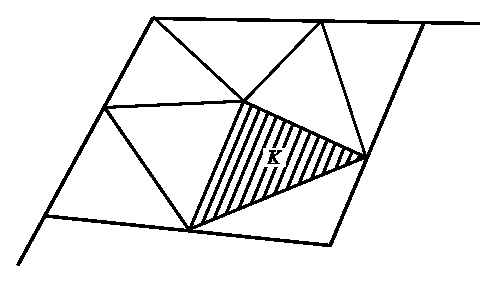
\includegraphics{figures/fig3.1.eps}
\centerline{\bf Fig. 3.1.}
\end{figure}

A continuous flow is described by a simple wave whenever it is adjacent to constant state. An inward bend (Fig. 3.1(a)) causes the characteristics to form a cusped envelope and hence a shock. An outward bend (Fig. 3.1(b)) has a continuous rarefaction wave possibly ending at zero density\pageoriginale and the escape velocity which, by Bernoulli's law, is equal to $q^*$. A sharp straight bend yields a rarefaction wave or a straight shock (Figures 3.2 (a) and 3.2(b)).
\begin{figure}[H]
\centering
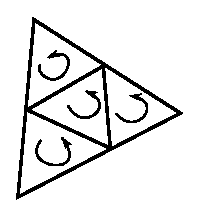
\includegraphics{figures/fig3.2.eps}
\centerline{\bf Fig. 3.2.}
\end{figure}

These problems are easily solved by noting that the image of the rarefaction wave if a characteristic in the $(u,v)$-plane and the image of the possible states behind the shock is given by a so called {\em shock polar}. It is convenient to look at these in $(\theta ,q)$ - plane, where $\theta$ is the flow angle $\tan^{-1}(v/u)$.

\section{Shock polar}\label{chap3:sec3.4}
From the discontinuity conditions in the form 
\begin{align*}
& [\rho u] dy / dx - [\rho v] = 0, \\
& [u] + [v] dy/ dx = 0,
\end{align*}
where\pageoriginale $dy/dx$ is the slope of the shock, we find that with an initial state $(q_o, 0)$ with $\rho_o = \rho (q_o)$, if the state behind the shock is ($q \cos \theta$, $q \sin \theta$), then
\begin{equation*}
q \cos \theta = \frac{\rho q^2 + \rho_o q^2_o}{q_o (\rho + \rho_o)}.
\tag{3.12}\label{eq3.12}
\end{equation*}

In the limit of a weak shock, we note that a shock can become weak in two ways: either the shock becomes characteristic or the flow on both sides becomes sonic.
To see this, we set
$$
F = \rho q, \; F_o = \rho_o q_o, \; F/F_o = 1 + \delta G \quad \text{and} \quad q/ q_o = 1 + \delta p.
$$
Then we obtain from (\ref{eq3.12})
$$
\cos \theta = 1 + \frac{\delta p \cdot \delta G}{2 + \delta p + \delta G}
$$
or 
$$
\sin^2 \frac{\theta}{2} = - \frac{1}{2} \; \frac{\delta p \delta G}{2 + \delta p + \delta G}.
$$
To a first order approximation, we have
$$
\delta G = \delta p \cdot \rho_o \cdot d F / dq .
$$
Hence, if the shock is weak we have $\theta \to 0$ and $\delta p \to 0$, and we obtain
$$
\theta^2 = (\delta p)^2 (-dF / dq),
$$
and the shock is characteristic with 
$$
\theta = \pm \delta p (-d F / dq)^{1/2},
$$
provided $dF/dq \neq 0$. However, if the velocities on both sides of\pageoriginale the shock are close to sonic, if we approach the limit appropriately:
$$
\theta^2 = (\delta p)^3.
$$
Note that in the normal shock case $\theta = 0$ and $\delta G \equiv 0$. The shock polar for the polytropic case is as illustrated in Fig. 3.3 (See Bers \cite{key2}).
\begin{figure}[H]
\centering
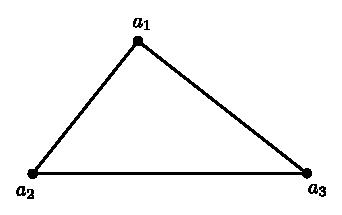
\includegraphics{figures/fig3.3.eps}
\centerline{{\bf Fig. 3.3.} SHOCK POLAR}
\end{figure}

An important problem is the detached problem. Suppose a projectile or wing is moving in a fluid with supersonic speed. If the projectile (or wing) is round the speed vanishes at the tip (stagnation point). There is a shock in front, {\em not} an attached shock. The shock is curved and the flow is constant in front because of the curvature behind the shock, the flow is not strictly isentropic or irrotational. If the shock strength is moderate a situation that occurs if the speed at infinity is not too high we may still use the conditions of irrotationality and isentropy. Then there is a subsonic region around the nose.
\begin{figure}[H]
\centering
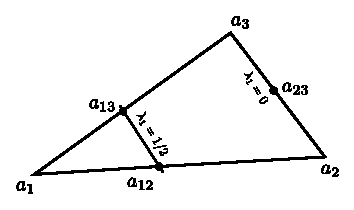
\includegraphics[scale=0.8]{figures/fig3.4.eps}
\centerline{{\bf Fig. 3.4.} DETACHED SHOCK OVER A BLUFF BODY}
\end{figure}\pageoriginale

The problem is to solve (\ref{eq3.1}) and (\ref{eq3.3}), a mixed system, with boundary condition $udy - vdx = 0$ on the object. The shock is a free boundary in the flow represented in the $u,v$ place by the shock polar. From (\ref{eq3.12}) one sees that the flow behind the shock is subsonic on the axis, so there is a region of subsonic flow. However, like the nozzle flow discussed in \S 12 there are no transonic difficulties such as those described in \S 7-11. See Bauer et al. \cite{key1}.

\section{Equations in the hodograph plane}\label{chap3:sec3.5}
By the hodograph plane, we shall mean either $(u,v)$ or $(q,0)$ or even $(\sigma (q), \theta)$ plane, whichever is convenient since they correspond to simple mappings except near $q = 0$. However near $q=0$,\pageoriginale the equation for the potential $\phi$ behaves like $\Delta \phi =0$ and we have a very complete understanding of the flow. The special function $\sigma (q)$ is chosen to simplify the equations. From (\ref{eq3.8}), we obtain
$$
q^{-1} e^{\sqrt{-1} \theta} (d \phi + \frac{\sqrt{-1} d\psi}{\rho}) = dx + \sqrt{-1} dy. 
$$
Hence the left hand side is a perfect differential. Considering $\phi$, $\psi$ as functions of $\sigma$, $\theta$, where $\sigma = \sigma (q)$, we find 
$$
q^{-1} e^{\sqrt{-1}\theta} (\phi_\theta + \frac{\sqrt{-1} \psi_\theta}{\rho}) d \theta + q^{-1}  e^{\sqrt{-1} \theta} (\phi_\sigma + \frac{\sqrt{-1} \psi_\sigma}{\rho}) d\sigma
$$
is a perfect differential. This requires
$$
\{q^{-1} e^{\sqrt{-1} \theta} (\phi_\theta + \frac{\sqrt{-1} \psi_\theta}{\rho})\}_\sigma = \{ q^{-1} e^{\sqrt{-1} \theta} (\phi_\sigma + \frac{\sqrt{-1} \psi_\sigma}{\rho}) \}_\theta.
$$
Thus,
\begin{align*}
& (q^{-1})_\sigma\phi_\theta + \rho^{-1} q^{-1} \psi_\sigma = 0, \tag{3.13}\label{eq3.13}\\
& (\rho^{-1} q^{-1})_\sigma \psi_\theta - q^{-1} \phi_\sigma = 0. \tag{3.14}\label{eq3.14}
\end{align*}
For the transonic range, it is convenient to introduce
$$
\sigma = \int\limits^q q^{-1} \rho \; d q.
$$
Then  equations (\ref{eq3.13}) and (\ref{eq3.14}) reduce to 
$$
\phi_\theta = \psi_\sigma,
$$
and
$$
\phi_\sigma = - K(\sigma) \psi_\theta,
$$
where
$$
K(\sigma) = \frac{1}{\rho^3 q^2} \frac{d(\rho q)}{dq}
$$\pageoriginale 
is a function of $\sigma$ only. Thus
\begin{equation*}
K(\sigma) \; \psi_{\theta \, \theta} + \psi_{\sigma \sigma} = 0.  \tag{3.15}\label{eq3.15}
\end{equation*}
Note that the equation is elliptic or hyperbolic according as $K(\sigma)$ is positive or negative, i.e., as $\sigma$ is positive or negative. Note also that the characteristics of (\ref{eq3.15}) are given by
\begin{equation*}
\theta = \pm \int\limits^\sigma_o\sqrt{-K(\sigma)} d \sigma + \text{ constant}. 
\tag{3.16}\label{eq3.16}
\end{equation*}

\medskip
\noindent{\textbf{The Legendre Transformation: }} In solving perturbation problems, it will be convenient to use the Legendre transformation which we introduce now. Recall equations (\ref{eq3.1a}) and (\ref{eq3.9}). If we regard $x,y$ as functions of $u,v$ the equations reduce to 
\begin{equation*}
x_v - y_u = 0\tag{3.17}\label{eq3.17}
\end{equation*}
$$
(c^2 - u^2 ) y_v + uv (x_v + y_u) + (c^2 -v^2) x_u = 0.
$$
By (\ref{eq3.17}), there is a function $\chi(u,v)$, {\em Legendre transformation}, satisfying
$$
x = \chi_u, \; y = \chi_v. 
$$
The relation between the potential $\phi$ and $\chi$ is then given 
by 
$$
\phi = xu + yv -\chi
$$
as is easily seen. Similarly, we can introduce a {\em Legendre transformation } $\tilde{\chi}$ such that the stream function $\psi$ can be written as
$$
\psi = - \rho x v + \rho y u - \tilde{\chi}. 
$$\pageoriginale 
It is clear that we can consider both $\chi, \tilde{\chi}$ as functions of $q$, $\theta$.

Combining the definitions of $\chi, \tilde{\chi}$ with (\ref{eq3.8}), we find that 
\begin{align*}
 d \chi  & = x du + ydv = x (\cos \theta dq-q \sin \theta d\theta) + y (-\sin \theta dq - q \cos \theta d \theta),\\
d\tilde{\chi} & = yd (\rho u) - x d (\rho v) = y (\cos \theta \frac{d(\rho q)}{dq} dq - \sin \theta \cdot \rho q d \theta)\\
& \qquad \qquad -x (-\sin \theta \frac{d(\rho q)}{dq} dq - \cos \theta \rho q \; d\theta). 
\end{align*}
From which it follows that 
$$
\chi_\theta = - (\frac{d(\rho q)}{dq})^{-1} \tilde{\chi}_q, \quad \chi_q = (\rho q)^{-1} \tilde{\chi}_\theta. 
$$
We set
$$
d\hat{\sigma} = dq/\rho q \quad \text{and} \quad \hat{K} = \rho q \frac{d(\rho q)}{dq}
$$
and the equations become
$$
\hat{K} \chi_\theta = - \tilde{\chi}_{\hat{\sigma}}, \; \chi_{\hat{\sigma}} = \tilde{\chi}_\theta, 
$$
where $\hat{K}$, $\hat{\sigma}$ are not the same as $K$ and $\sigma$ but have the same basic properties.

Furthermore,
\begin{equation*}
\hat{K} \chi_{\theta \theta} + \chi_{\hat{\sigma} \hat{\sigma}} = 0. 
\tag{3.18}\label{eq3.18}
\end{equation*}
We shall use  this equation later in connection with perturbation problems.

See Bers \cite{key2} for more details on these equations and for early work on subsonic and transonic theory.

\section{Small Disturbalce equation}\label{chap3:sec3.6}
Von Karman's model\pageoriginale nonlinear mixed equation
\begin{equation*}
\phi_x  \phi_{xx} + \phi_{yy} = 0, \tag{3.19}\label{eq3.19}
\end{equation*}
elliptic for $\phi_x > 0$, hyperbolic for $\phi_x < 0$, can be derived from (\ref{eq3.8}) by expanding $\theta$ about `$0$' and $q$ about the sonic value $c_o$. From
$$
\rho d \phi + \sqrt{-1} d \psi = \rho q e^{-\sqrt{-1} \theta} dz
$$
we have with $\phi = c_o x - \phi$, $\psi = \rho_o c_o y+ \psi$,
\begin{align*}
& (\rho_o + \rho - \rho_o) \; (c_o dx - d\phi) + i (\rho_o c_o dy + d\psi)\\
& \qquad = (\rho_o q_o + \frac{1}{2} \frac{d^2 (\rho q)}{dq^2} \mid_o (q-c_o)^2 + \ldots) \; (1 - i \theta + \ldots) dz
\end{align*}
so that from the highest order terms
$$
-\rho_o d \phi  + id \psi = [A(q-c_o)^2 - \rho_o q_o i \theta] dz - B (q-c_o) dx,
$$
where 
$$
A = \frac{1}{2} d^2 (\rho q) / dq^2 \mid_o \quad\text{and} \quad  B = d\rho /dq|_o \cdot c_o.
$$
Here, we have used 
$$
d(\rho q ) / d q|_o = 0 \quad \text{and} \quad q_o = c_o. 
$$
Thus
\begin{align*}
\rho_o \phi_x & = B (q-c_o) - A(q-c_o)^2\\
\psi_x & = - \rho_o q_o \theta\\
-\rho_o \phi_y & = \rho_o q_o \theta\\
\psi_y & = A (q-c_o)^2.
\end{align*}
The small\pageoriginale disturbance equations are obtained by eliminating $\theta$, $q$ and thus 
\begin{align*}
& \phi^2_x = \rho^{-2}_o B^2 A^{-1} \psi_y, \text{ to first order in } \psi_y \propto (q-c_o)^2,\\
& \rho_o \phi_y = \psi_x.
\end{align*}
But $A < 0$ so that after rescaling  ($x \to x$ and $y \to (-\frac{1}{2} \rho^{-1}_o B^2 A^{-1})^{-1/2} y$) we obtain
\begin{align*}
& \phi^2_x = (-\frac{1}{2} \rho^{-1}_o B^2 A^{-1})^{1/2} (-2 \rho^{-1}_o) \psi_y, \\
& \rho_o (-\frac{1}{2} \rho^{-1}_o B^2 A^{-1})^{-1/2} \phi_y = \psi_x. 
\end{align*}
These equations in turn yield (\ref{eq3.19}).

On the other hand, by expanding the hodograph equations we obtain
\begin{align*}
\sigma \phi_\sigma & = -\psi_\theta\\
\phi_\theta & = \psi_\sigma. 
\end{align*}

\section{Transonic flow}\label{chap3:sec3.7}
We limit our discussion to a few problems centered around transonic wing flow.

The first question is whether we can find a wing shape which at a prescribed subsonic speed at infinity has a smooth flow. Experimental observation suggested in the forties that perhaps such a steady flow did not exist as the speed came close to sonic at infinity and locally supersonic in a region next to wing. However, Lighthill \cite{key25} showed how to construct such a wing shape. But this wing was not\pageoriginale constructed possibly because the prevailing sense was that in any case it would be unstable. Frankl' and Guderley, \cite{key10}, \cite{key16}, proposed that the explanation for the instability lay in the fact that the boundary value problem was ill-posed in the sense of Hadamard if the flow was required to be smooth. This we proved by the author \cite{key29}. 

The implication was that in general flows with transonic regions would have shocks, not detached as in supersonic flow but arising in the supersonic region or cutting it off. This is in fact the case and the shocks have a strong effect on the drag. However, this effect is much less than the drag produced at supersonic speeds by the datached shocks. So that it has proved very useful to use such wings. In \cite{key33}, Nieuwland has designed an algorithm for finding, not a transonic wing, but a smooth transonic cross-sections.

In the following sections, we shall discuss the relevant boundary value problems and the related general theory of mixed equations. Then we shall describe the design of aerofoil shapes developed by Garabedian et al., and the method introduced by Murman and Cole for finding the flows at off design Mach numbers.

\section[General theory of boundary value...]{General theory of
  boundary value problems for mixed equations}\label{chap3:sec3.8} 
The mixed equations were first investigated by Tricomi, see
\cite{key36}, for the equation that bears his name and is the
hodograph equation for the small disturbance equation: 
\begin{equation*}
\sigma \psi_{\theta \theta} + \psi_{\sigma\sigma} = 0, \tag{3.20}\label{eq3.20}
\end{equation*}\pageoriginale
see the end of \S\ 7.

A sample theorem on a boundary value problem which illustrates that the standard Dirichlet problem would be over determined is:
\begin{figure}[H]
\centering
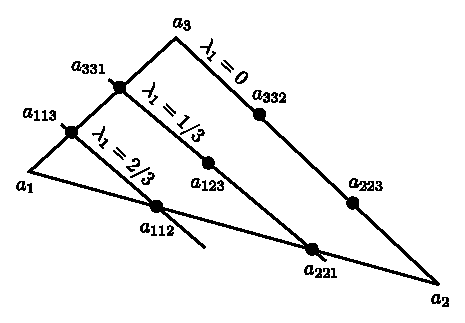
\includegraphics{figures/fig3.5.eps}
\centerline{{\bf Fig. 3.5.} TRICOMI PROBLEM}
\end{figure}

\begin{theorem*}
Suppose $\psi$ satisfies (\ref{eq3.20}), where $\psi$ is prescribed on the curve $C_3$ and the characteristic $C_2$. Let $D$ be the region enclosed by the curves $C_3, C_1$ and $C_2$ ($C_1$ is also a characteristic). Suppose the are $C_3$ is star-like\footnote{This condition means, as a point moves along $C_3$  inthe counterclockwise direction the angle which it makes the $\theta$-axis is increasing.} with respect to the origin:
$$
\theta d \sigma - \sigma d \theta >0.
$$
Under these conditions, the solution is unique for $\psi_\sigma, \psi_\theta$ continuous throughout the closure of $D$ (See Garabedian \cite{key13}).
\end{theorem*}

It is reasonable to expect such a theorem. Consider the still simpler mixed equation (Lavrente'v, Bitsadze \cite{key22}).
\begin{equation*}
(sgn \; \sigma) \psi_{\theta \theta} + \psi_{\sigma\sigma} = 0
\tag{3.21}\label{eq3.21}
\end{equation*}
and the same boundary data. Here $C_1$ and $C_2$ are the straight characteristics. Let $F$ be the value of $\psi$ on $\sigma = 0$.\pageoriginale Then $G = \partial \psi / \partial \sigma | \sigma = 0$ found by solving an elliptic problem is a linear functional of $F$, in $\sigma \geqq 0$. On the other hand solving the wave equation, for $\sigma < 0$, one finds that the data on $C_2$ alone determine another linear relation between $F$ and $G$. It is reasonable to expect that one can eliminate $G$ and solve for $F$ uniquely. Then $\psi$ is easily seen to be unique.

There are a variety of methods for proving the theorem and also establishing the existence of the solution. The method we shall use is by an estimate. Without loss of generality, we can consider the nonhomogeneous equation with homogeneous boundary data. We rewrite the equation as a system by setting
$$
\omega = (\omega_1 , \omega_2)^t \quad \text{with} \quad \omega_1 = \psi_\theta, \; \omega_2 = \psi_\sigma
$$
and thus 
\begin{equation*}
\begin{split}
&  A \omega_\theta + B \omega_\sigma = f\\
& \omega_1 d\theta + \omega_2 d\sigma = 0 \quad \text{on}\quad C_2 + C_3\\
\end{split}\tag{3.22}\label{eq3.22}
\end{equation*}
where 
\begin{equation*}
A = \begin{pmatrix}
\sigma & 0\\
0 & -1
\end{pmatrix} \; B = \begin{pmatrix}
0 & 1\\
1 & 0
\end{pmatrix}
\tag{3.23}\label{eq3.23}
\end{equation*}
which is a symmetric system.

We seek a matrix $C$ with a certain property: Take the `scalar product'  of (\ref{eq3.22}) with $C$, where $AC$ and $BC$ are symmetric. Integrate by parts over the domain $D$. Apply the boundary condition. Choose $C$ so that the boundary\pageoriginale and area integrals are positive definite. Denote the area integral by $Q(\omega, \omega)$. Then
$$
Q(\omega, \omega) \quad (f, C\omega), 
$$
where $(,)$ is defined for any two column vector functions
$$
f = (f_1 , f_2)^t, \; g = (g_1, g_2)^t
$$
by
$$
(f,g) = \iint\limits_D (f_1 g_1 + f_2 g_2) dx \; dy.
$$
Thus if $f \equiv 0$ then $\omega \equiv 0$ which proves uniqueness.

We now proceed to find $C$. If
$$
C = 
\begin{pmatrix}
c_{11} & c_{12}\\
c_{21} & c_{22}
\end{pmatrix}
$$
we find 
$$
(C\omega, A \omega_\theta) = (A C \omega, \omega_\theta) = \frac{1}{2} (AC\omega, \omega) - \frac{1}{2} ((AC)_\theta \omega, \omega), 
$$
provided $AC$ is symmetric, i.e., $\sigma c_{12} = - c_{21}$, and 
$$
(C\omega, B\omega_\sigma) = \frac{1}{2} (BC\omega, \omega)_\sigma - \frac{1}{2} ((BC))\sigma \omega, \omega),
$$
provided $BC$ is symmetric, i.e. $c_{11} = c_{22}$. Hence the boundary term is, by Green's theorem,
$$
\frac{1}{2} \int \omega^2_1 \sigma (bd \sigma + cd \theta) + 2 \omega_1 \omega_2 (\sigma cd \sigma - b d \theta) - \omega^2_2 (bd \sigma - cd\theta). 
$$
Here $c_{11} = c_{22} = b$ and $c_{12} = c$. 

The contribution to this term from $C_2  + C_3$ where $\psi = 0$ and we may write
\begin{equation*}
\omega_1 = \alpha d\sigma, \; \omega_2 = - \alpha d \theta\tag{3.25}\label{eq3.25}
\end{equation*}
is\pageoriginale
$$
\frac{1}{2} \int\limits_{C_2 + C_3} \alpha^2 (bd\sigma - cd\theta) \; (\sigma d \sigma^2 + d \theta^2). 
$$
And the integral on the characteristic $C_1$ where $d\theta + \sqrt{-\sigma} d\sigma = 0$ is
$$
-\frac{1}{2} \int\limits_{C_1} \{ (\sqrt{-\sigma} \omega_1 - \omega_2)^2 \; (b + c\sqrt{-\sigma})\} d \sigma.
$$

Hence to fulfil the required positivity $C$ must satisfy:

$(AC)_\theta + (BC)_\sigma$ is a negative definite matrix
\begin{align*}
& bd \sigma - cd \theta \geq 0 \quad \text{on} \quad C_2 + C_3\\
&  (b+c\sqrt{-\sigma}) d \sigma \leq 0 \quad \text{on} \quad C_1. 
\end{align*}
We then find the explicit requirements,
\begin{align*}
\sigma b_\theta - (\sigma c)_\sigma \leqq 0\\
-b_\theta + c_\sigma \leqq 0 \tag{3.26}\label{eq3.26}\\
(\sigma c_\theta + b_\sigma)^2 \leqq (\sigma b_\theta - (\sigma c)_\sigma) (-b_\theta + c_\sigma)  
\end{align*}
 in $D$ and the boundary conditions
\begin{gather*}
(bd\sigma -cd\theta) \; (\sigma d\sigma^2 + d\theta^2) \leqq 0 \quad\text{on} \quad C_2 + C_3\\
(b -\sqrt{-\sigma} c) \geqq 0 \quad \text{on}\qquad  C_1
\end{gather*}
The choice $b = \theta$, $c = \sigma$ for $\sigma \geq 0$, $c=0$ for $\sigma \leqq 0$ satisfies these requirements. This completes the uniqueness theorem. Note that the requirements would also be fulfilled if $C_2$ was not characteristic but satisfied only
$\sigma d \sigma^2 + d\theta^2 \geq 0$\pageoriginale and that the star-shaped condition on $C_2$ could be freed up by changing $b$ and $c$.

A weak solution $\omega \in H_*$ of (\ref{eq3.22}) and (\ref{eq3.25}) satisfies
$$
-(Lv, \omega) = (v,f)
$$
for all smooth vectors $v$ such that
$$
v_1 = 0 \quad \text{on} \quad C_2 + C_3
$$
and, since the matrix $A + \sqrt{-\sigma} B$ is singular, such that 
$$
v_2 -v_1 \sqrt{-\sigma} = 0 \quad \text{on}\quad C_1,
$$
where $L = A \; \partial / \partial \theta + B \partial /\partial \sigma$ and $H_*$ is defined below.

This is the adjoint problem. To use the projection theorem it would suffice to find a Hilbert space for which $(v,f)$ would be a bounded linear functional of $Lv$ for $v$ satisfying boundary conditions. But $(v,f)$ is a bounded linear functional in $v$ in some weighted $L^2$-space and $f$ in its corresponding space. So, we have to find an appropriate space in which $v$ is bounded in terms of $Lv$ if 
\begin{equation*}
v_1 = 0 \quad \text{on}\quad C_1 + C_2 + C_3. 
\tag{3.27}\label{eq3.27}
\end{equation*}
We proceed to the details.

Let $H_*$ be the Hilbert space of all pairs of measurable functions $u = (u_1, u_2)$ for which the norm
$$
|| u ||^2_* = \iint\limits_D (ru^2_1 + u^2_2) d \theta \; d\sigma
$$
is finite; the inner product is given by 
$$
(u,v)_* = \iint\limits_D (ru_1 v_1 + u_2 v_2) d \theta \; d\sigma,
$$\pageoriginale
where $r^2 = \theta^2 + \sigma^2$.

Let $V$ be the set of all function $\omega = (\omega_1, \omega_2)$ with continuous derivatives and such that
\begin{align*}
 \omega & = (0,0) \quad \text{at} \quad  r=0, \\
\omega_1 & = 0\quad \text{on} \quad C_1 + C_2 + C_3, 
\end{align*}
and 
$$
\iint\limits_D (\frac{1}{r} (L\omega)^2_1 + (L\omega)^2_2) d\theta \; d\sigma < \infty
$$
Let $H^*$ denote the Hilbert space of all measurable functions $u = (u_1, u_2)$ for which
$$
|| u ||^* = \{\iint\limits_D (\frac{1}{r} u^2_1 + u^2_2) d \theta \; d\sigma\}^{1/2}
$$
is finite; the inner product is
$$
(u,v)^* = \iint\limits_D (\frac{1}{r} u_1 v_1 + u_2 v_2) d\theta \; d\sigma. 
$$
Note that $LV \subset H^*$. We now state the following. 

\begin{theorem*}
There exists a weak solution of (\ref{eq3.22}) and (\ref{eq3.25}) for every $f \in H^*$. 

To prove the theorem we require the following lemma which will be proved later.
\end{theorem*}

\begin{lemma*}
For all $v \in V$, $f \in H^*$
$$
|(v,f)| \leqq B||Lv||*||f||^*,
$$
where $B$ is a constant. 
\end{lemma*}

\medskip
\noindent{\textbf{Proof of the Theorem; }}
For $v \in V$\pageoriginale define
$$
G(Lv) = (v,f).
$$
By the lemma $G$ is bounded on $LV \subset H^*$. Thus by Hahn-Banach theorem $G$ can be extended to $H^*$ as a bounded linear functional. Thus by classical Riesz's representation theorem there is a $t \in H^*$ such that 
$$
(Lv,t) = (v,f) \quad \text{for all}\quad v \in V. 
$$
The function $\omega$ defined by $\omega_1 = -t_1 /\Omega$, $\omega_2 = - t_2$ will belong to $H_*$ and satisfies $-(Lv, \omega) = (v,f)$. Thus $\omega$ is the required weak solution and this completes the proof.

\medskip
\noindent{\textbf{Proof of the Lemma: }}
By Schwarz's inequality, we obtain
$$
|(v,f)| \leqq ||v||_* ||f||^*.
$$
Thus the proof will be complete if we prove the a-priori estimate
$$
||v||_* \leqq B||Lv||^*,
$$
where $B$ is a constant.

We proceed to do this, Set
\begin{equation*}
v = C \tilde{v}.   \tag{3.28}\label{eq3.28}
\end{equation*}
Again consider 
$$
(Lv, \tilde{v}) = (Av_\theta + Bv_\sigma, \tilde{v}) = (A(C\tilde{v})_\theta + B(C \tilde{v})_\sigma, \tilde{v}).
$$
Again by rearranging terms properly, we can integrate by parts. The boundary condition (\ref{eq3.7}) becomes $b\tilde{v}_1+ c \tilde{v}_2 =0 $. Set
$$
(Lv, \tilde{v}) = I_1 + I_2,
$$
where\pageoriginale $I_1$ is area integral and $I_2$ is surface integral. It is easy to see that if (\ref{eq3.26}) is satisfied then $I_1$ is positive definite; also $I_2$ is non-negative. Thus 
$$
|(Lv, \tilde{v})| \geqq I_1. 
$$
On the other hand, for any $\lambda > 0$,
$$
|(Lv, \tilde{v})| \leqq \lambda ||Lv||^{*^2} + \frac{1}{\lambda}||\tilde{v}||_*
$$
and hence
$$
I_1 \leqq \lambda || Lv||^{*^2} + \frac{1}{\lambda} ||v||^2_*, \quad \lambda > 0.
$$
Thus if $||\tilde{v}||_*$ can be estimated in terms of $I_1$ then by choosing $\lambda$ sufficiently large, we can estimate $||\tilde{v}||_*$ in terms of $||Lv||^*$. For the same choice of $b$ and $c$ one can estimate $||\tilde{v}||_*$ in terms of $I_1$. This estimate is obtained by the same method as was used in the uniqueness theorem.

Once the existence of the weak solution has been established, one proceeds to determine whether it has in fact some better properties but we shall not do that here except to say that since the smoothness properties are local, elliptic methods suffice in elliptic regions, hyperbolic in hyperbolic regions, and that the solution is a strong solution everywhere.

For general description, see Morawetz \cite{key30}. See also Osher \cite{key35} for a different approach.

\section{The boundary value problems of transonic wing flow}\label{chap3:sec3.9}
The two most important boundary value problems for transonic wing flow are for the nonlinear solution and for the linearized flow about it.

In the\pageoriginale physical plane, the flow potential $\phi$ satisfies (\ref{eq3.10}), the boundary condition $\partial \phi / \partial n=0$ on the wing and at infinity, $\nabla \phi$ is prescribed. We know from incompressible flow that we need, for a well-posed problem, the additional condition (the Kutta-Joukowski condition) that the circulation at infinity adjusts itself so that the flow past a wing with a cusp at the trailing edge has finite velocity. For compressible flows by Bernoulli's law, no infinite velocity is possible any way and the circulation adjustment is chosen to prevent.

It is not unreasonable to anticipate that the problem is overdetermined on the basis of the boundary value problems discussed earlier. There are two possibilities: Shocks in general and special smooth solutions.

The problem with shocks for a general aerofoil has only been tackled numerically. There is some indication that its perturbation problem is well-posed, see Morawetz \cite{key27}. ]

There exist numerical codes (``analysis'' codes) for solving the\break
boundary value problem using artificial viscosity or penalty
methods. The original viscosity method of Murman and Cole \cite{key32}
is described in \S\ 12. It's basic ideas have been incorporated and
considerably modified by Jameson \cite{key18} and can now be used on
three dimensional problems. Bristeu et al. \cite{key4} has used finite
elements and a penalty method.   

The lag of the theory behind numerical experiment is not suprising especially when one realizes how limited the theory is with respect to one dimensional flow.


In the\pageoriginale case of no shocks, the problem can be looked at in the hodograph plane. under the hodograph transformation, see \S\ 5, the problem transforms into a free boundary value problem\footnote{This approach has been explored by Brezis and Stampacchia \cite{key3} for subsonic flows}. Consider the symmetric wing section which has a singly curved image in the hodograph plane. The equation, say for $\psi$, (\ref{eq3.15}), is linear. There is a prescribed singularity at the image point of the point at infinity. The boundary condition $\psi=0$ is imposed on the axis $\theta = 0$ and the unknown image of the wing, see Fig. 3.6. But there is a second boundary condition because the flow angle $\theta$ is a prescribed function of the arc length on the wing. Using (\ref{eq3.8}), this yields, on the free boundary,
$$
d\phi = q(\sigma) e^{\sqrt{-1} \theta} (dX (\theta) + \sqrt{-1} dY (\theta)),
$$
where $x = X(\theta)$, $y = Y(\theta)$ describe the wing. This is only one condition since $\tan \theta = dY / dX$. Then using
$$
d\phi = \psi_\sigma d \theta - K \psi_\theta d \sigma
$$
we have the extra condition on $\psi$:
$$
-\psi_\sigma d \theta + K \psi_\theta d \sigma = q(\sigma).
$$

Solutions for special shapes known as {\em super-critical} airfoils corresponding to smooth flow pasta wing can be found. One solves the boundary value problem without the last condition (3.31) using some smooth boundary and a well posed problem. But we know from \S\ 8 that we cannot expect to solve the problem with full Dirichlet conditions. Instead use the following procedure:
\begin{figure}[H]
\centering
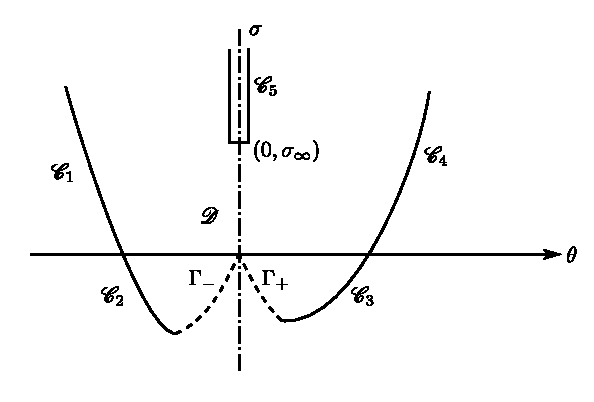
\includegraphics{figures/fig3.6.eps}
\centerline{\bf Fig. 3.6.}
\end{figure}\pageoriginale

Solve the boundary value problem:
\begin{align*}
& K \psi_{\theta \theta} + \psi_{\sigma \sigma} = 0 \quad \text{in}\quad D\\
& \psi = 0 \quad \text{on} \quad C_1 + C_2 + C_3 + C_4 + C_5, 
\end{align*}
with prescribed singularity at $(0, \sigma_\infty)$. Here $C_1+ C_2$ and $C_3+C_4$ are smooth arcs satisfying 
$$
\sigma d\sigma^2 + d\theta^2 \geqq 0,
$$
and $C_5$ is a slit on $\sigma$-axis s.t. $\sigma_\infty \leqq \sigma < \infty$ on $C_5$. 

The rest of the boundary of $D$ consists of two characteristics $\Gamma_-$ and $\Gamma_+$ issuing from the origin until $C_2$, $C_3$ are intersected. It can be shown by the methods of the preceding section that this is a well-posed problem. The singularity at $(0, \sigma_\infty)$ is a bit messy (see Gilbarg \cite{key14}; but for our purposes it suffices to treat it like the incompressible flow singularity which would require taking $K(\sigma_\infty) = 1$ and 
\begin{equation*}
\psi_\theta - \sqrt{-1} \psi_\sigma - A (\phi + \sqrt{-1} \sigma)^{3/2} = 0 (|\phi +\sqrt{-1} \sigma |^{1/2}) \tag{3.32}\label{eq3.32}
\end{equation*}\pageoriginale
where $A$ is related to the prescribed speed of the wing).

We now have part of a flow and part of a supercritical wing image $(C_1 + C_2 + C_3 + C_4)$ in the hodograph plane. To choose the wing, we continue the solution $\psi$ across the characteristic gap, $\Gamma_+$ and $\Gamma_-$, by solving the appropriate Goursat problem. It is not unreasonable to expect that there will be curve joining $C_2$ to $C_3$ on which $\psi=0$ especially if the hyperbolic region is small. At this stage we have solved the hodograph problem. The next stage is to find the physical image using (\ref{eq3.8}). A short calculation shows that this will fail if $K(\sigma)\psi^2_\theta + \psi^2_\sigma$ changes sign (a limiting line occurs where $K(\sigma) \psi^2_\theta + \psi^2_\sigma = 0$). But again for sufficiently small hyperbolic regions this does not happen and we do in fact find a physical flow.

In the next section, we describe the method used by Garabedian to generate smooth flows. Fung et al. \cite{key12} has used the idea of finding first a purely subsonic flow with a sonic line separating two subsonic regions adjusting the equation of state and then continuing the flow from the sonic line into the smaller region using the right equation of state and finding a new profile.

There are other possibilities for generating supercritical wing sections all involving some form of unique continuation. 

Having\pageoriginale constructed a smooth flow and a wing section, one way or another, one asks what happens to this flow when it is a disturbed say by changing its tilt (angle of attack) or by changing its speed at infinity (Mach number). The evidence both numerical and experimental is that a shock develops at the rear sonic point on the wing profile. It increases the drag (and hence the fuel consumption). Theoretically there are no results on the nature of this shock flow.

\section{Perturbation boundary value problem}\label{chap3:sec3.10}
It would be useful to know what flows close to supercritical (smooth transonic) flows look like. First one looks at the general perturbation problem assuming that the nearby flow is smooth. This leads to a contradiction. Then one asks what actually happens.

First, the perturbation equation has to be determined. The direct method from equations (\ref{eq3.9}) is tedious. Instead, for the Legendre potential
$$
\chi (u,v) = xu + yv - \phi (x,y)
$$
we see that the perturbation Legendre potential $\delta \chi$ satisfies
$$
\delta \chi = \delta x. u + \delta y. v - \phi_x \delta x - \phi _y \delta _y - \delta \phi
$$
in terms of a perturbation potential $\delta \phi$ and the perturbations $\delta x$, $\delta y$. But $\phi_x = u$ and $\phi_y =v$ so that $\delta \chi = - \delta \phi$ to first order. Thus, in the hodograph variables $\theta$, $\hat{\sigma}$ of the {\em undisturbed flow} since $\delta \chi$ satisfies (\ref{eq3.18}) so does $\delta \phi$. Thus
\begin{equation*}
\hat{K} (\delta \phi)_{\theta \theta} + (\delta \phi)_{\hat{\sigma} \hat{\sigma}} = 0. 
\tag{3.33}\label{eq3.33}
\end{equation*}\pageoriginale
On the perturbed boundary given by 
$$
y = Y (x) + \delta Y (x)
$$
we find 
$$
\frac{\partial \phi}{\partial n} (x,Y + \delta Y) + \frac{\partial}{\partial n} (\delta \phi) = 0,
$$
or to first order 
\begin{equation*}
\frac{\partial}{\partial n} \delta \phi - (\frac{\partial}{\partial n} \phi_y) \delta Y = 0. \tag{3.34}\label{eq3.34}
\end{equation*}
At infinity, if there is a change in Mach number at infinity, there is a prescribed singularity of order $3/2$ as in the unperturbed case; see (\ref{eq3.32}).

If we restrict ourselves to solutions with continuous derivatives (no shocks) then one finds by using the methods of the first section of this chapter, that the problem is ill-possed if we fix the Mach number and change the profile, i.e., $\delta Y \neq 0$. For the symmetric profile see Morawetz \cite{key28}, for the non-symmetric case Cook \cite{key5}. Very partial results exist if we change Mach number, Morawetz \cite[III]{key29}.

The simplest proof amounts to showing that the solution is uniquely determined up to a one parameter family by the prescribed data ourside a ``characteristic gap'', i.e., by data on $C_1+ C_2 + C_3 + C_4$, see Fig. 3.6, since $\hat{\sigma} = \hat{\sigma} (\sigma)$. Therefore the function $\delta Y(x)$ cannot be arbitrary in the gap since $\delta \phi$ is determined by unique continuation from $\Gamma_+$, $\Gamma_-$. A more elaborate proof shows that $\delta Y (x) = 0$ in the gap if $\delta Y \equiv 0$ on $C_1+ C_2 + C_3 + C_4 + C_5$.

The next\pageoriginale question is how to find a well-posed perturbation problem that  represents a disturbance with shocks. The answer probably lies in finding a suitable singular perturbation for the case where on the whole boundary the value of $\delta Y$ is given arbitrarily. This might be accomplished by admitting singularities into the perturbation velocities at the places where shocks are expected, i.e., the points where the sonic line hits the profile. Thus the perturbation flow velocities would be a small variation on the unperturbed flow velocities but not right at the sonic points on the boundary. See \cite{key31} where such a singular Dirichlet problem is solved.

\section{Design by the method of complex characteristics}\label{chap3:sec3.11}
The method of complex characteristics has been introduced and used successfully by Bauer et at \cite{key1}, in the computation of flows and profiles. It began with the computation  of flows with Mach number greater than one at infinity where the object was to determine the subsonic flow behind an analytical shock, see \S\ 4. Its full strength came in the computation of supercritical airfoils, i.e., transonic but shock free with some Mach number less than one at infinity. We sketch here the principles involved in one of the early computations.

We are given a velocity at infinity for a flow. The object is to find an airfoil and a smooth flow past it with this velocity at infinity and with somewhat indefinitely specified characteristics:
\begin{itemize}
\item[{\rm (i)}] a large\pageoriginale supersonic region,

\item[{\rm (ii)}] a large decrease in the pressure (a large increases in the velocity) to control boundary layer separation on the forward end, and 

\item[{\rm (iii)}] a subsonic cusped trailing edge with the streamline from the upper surface meeting the one from the lower surface smoothly.
\end{itemize}

In the most recent work the object has been to specify the speed as a function of arc length along the airfoil but we will not describe this.

We write the equations of motion (\ref{eq3.3}) and (\ref{eq3.9}) as
$$
SU_x + TU_y = 0,
$$
where 
$$
U = 
\begin{pmatrix}
u\\v
\end{pmatrix} \; 
S = 
\begin{pmatrix}
c^2 - u^2 & -uv\\
0 & 1
\end{pmatrix} \quad \text{and} \quad  
T = 
\begin{pmatrix}
-uv & c^2 - v^2\\
-1 & 0
\end{pmatrix}
$$
and put this system in characteristic form formally. This yields the characteristic equations
\begin{equation*}
\begin{split}
y_\xi + \lambda_+ x_\xi & = 0, \quad u_\xi - \lambda_- v_\xi  =0,\\
y_\eta + \lambda_- x_\eta & = 0, \quad u_\eta -\lambda_+ v_\eta = 0,
\end{split} \tag{3.35}\label{eq3.35}
\end{equation*}
where 
$$
\lambda_{\pm} = \frac{uv \pm c \sqrt{q^2 -c^2}}{c^2 -u^2}. 
$$
Thus in the subsonic region where $q^2 < c^2$ the characteristics are complex. Note that $\xi$, $\eta$ are functions of $u,v$.

\begin{claim*}
$\xi$, $\eta$ may\pageoriginale be chosen so that in the real plane the solution is real. 
\end{claim*}

\begin{proof}
Let $\omega = u - \sqrt{-1} v$, $\omega^* = u + \sqrt{-1} v$. Suppose $\xi = \xi (\omega, \omega^*)$ and write 
\begin{align*}
\lambda_+ (\omega, \omega^*) & = \lambda_1 (\omega, \omega^*) + \sqrt{-1} \lambda_2 (\omega, \omega^*)\\
\lambda_- (\omega, \omega^*) & = \lambda_1 (\omega, \omega^*) - \sqrt{-1} \lambda_2 (\omega, \omega^*),
\end{align*}
with $\lambda_1 = uv/ (c^2 - u^2)$, $\lambda_2 = c \sqrt{q^2 - c^2}$, $\re (q^2 -c^2) > 0$. If $u,v$ are real, then $\lambda_1$, $\lambda_2$ are real and 
$$
\lambda_+ (\omega, \omega^*) = \overline{\lambda_-(\bar{\omega}^*, \bar{\omega})}
$$
where a bar above denotes the complex conjugate. Hence
$$
u_\xi (\omega,\omega^*) = \lambda_- (\omega, \omega^*) v_\xi (\omega, \omega^*)
$$
and changing values of the variable $\omega \to \bar{\omega}^*$, $\omega^* \to \bar{\omega}$ and because $u$ and $v$ are real, we obtain
$$
\overline{u_\xi (\omega, \omega^*)} = \overline{\lambda_+ (\omega, \omega^*)} \; \; \overline{v_\xi (\omega, \omega^*)}
$$
or 
$$
u_{\bar{\xi}} (\omega, \omega^*) = \lambda_+ (\omega, \omega^*) v_{\bar{\xi}} (\omega, \omega^*) . 
$$
This shows $\eta = \bar{\xi}$ is a possible characteristic variable in the subsonic region. 
\end{proof}

\medskip
\noindent{\textbf{A simple example: }}
Consider the Cauchy Riemann equations
\begin{align*}
u_x + v_y & = 0,\\
v_x - u_y & = 0. 
\end{align*}
Here\pageoriginale $\lambda_\pm = \pm \sqrt{-1}$ and therefore
\begin{align*}
y_\xi + \sqrt{-1} x_\xi & = 0, \quad u_\xi - \sqrt{-1} v_\xi = 0,\\
y_\eta - \sqrt{-1} x_\eta & = 0, \quad u_\eta + \sqrt{-1} v_\eta =0.
\end{align*}
So, $\omega = u - \sqrt{-1} v$, $\bar{\omega} = u + \sqrt{-1} v$ are characteristic co-ordinates.

\begin{note*}
Various problems could be solved in some limited region, for example, a Cauchy or Goursat problem. Now consider the elliptic region. There $\lambda_\pm$ are complex but the system remains valid. We consider $x,y,u,v$ as complex quantities. Note that $q^2 = u^2 + v^2$ and $c^2 (q)$ is an analytic function of $q$. Of course, we look for solutions which are real for real $x,y$.
\end{note*}

\begin{remarks*}
\begin{itemize}
\item[\rm{(1)}] Since the solution is analytic and independent of the path the number of actually used real variables can be reduced to {\em three}.

\item[\rm{(2)}] $\lambda_{\pm}$ are analytic in some slit domain because of the singularities at $q \pm c = 0$. This surface $q \pm c =0$ forms a two dimensional manifold in four dimensional space $(\omega, \omega^*)$. 
\end{itemize}
\end{remarks*}

We examine a difference scheme for a Goursat problem and first consider the real case. The difference scheme is given by 
\begin{align*}
& p(P) - p(Q) + \lambda_+ (Q) (q (P) - q(Q)) =0,\\
& p(P) - p (R) + \lambda_- (R) (q(P) - q(R))  = 0,
\end{align*}
where we use $p,q$ as variables. We want to solve for $p(P)$ and $q(P)$,\pageoriginale see Fig. 3.7.
\begin{figure}[H]
\centering
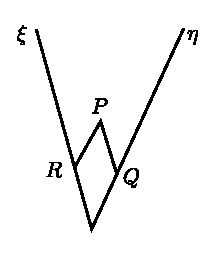
\includegraphics{figures/fig3.7.eps}
\centerline{\bf Fig. 3.7.}
\end{figure}

Here the data is prescribed on $\xi = 0$, $\eta = 0$ (For the Goursat problem see Garabedian \cite{key13} pp 118-119). We can solve for $p(P)$, $q(Q)$  provided $\lambda_+ \neq \lambda_-$ or equivalently $q^2 \neq c^2$. 

In the complex case, the same argument holds, but note that we should take $\overline{\Delta \xi} = \Delta \eta$ in the elliptic region. How do we guarantee that we have a real solution $x,y$ for real $u,v$? Note that the equations for $x,y$ are linear and they have real coefficients if $u,v$ are real. Hence $\re(x)$ and $\re(y)$ are solutions and these are real.

In practice, it has proved better to prescribe
\begin{align*}
x (\xi, \eta_o) & = f(\xi) + g(\eta_o)\\
x (\xi_o ,\eta) & = g(\eta) + f(\xi_o),
\end{align*}
and to get real solutions in the real plane by choosing $f(\xi) = \overline{g(\bar{\xi})}$.

The following problems arise:
\begin{itemize}
\item[{\rm (i)}] How to choose $f$ so that a stagnation point appears before a singularity? 

\item[{\rm (ii)}] How to\pageoriginale choose $f$ so that the streamlines of the profile join smooth\-ly at a trailing edge?
\end{itemize}

One usually chooses as a trial $f,g$ the corresponding data for the Cauchy-Riemann equations and then adjust.

\begin{remark*}
Existence up to a singular point follows  by a Cauchy-Kowa\-lew\-ski type of argument for a Goursat problem.
\end{remark*}

\section[Numerical solution with shocks: Off...]{Numerical solution
  with shocks: Off design\hfil\break computations}\label{chap3:sec3.12} 
We now consider the problem of computing flows for supercritical airfoils at off design, e.g., with different velocities at infinity than specified. This problem was open for a number of years and the first numerical solution of a nonlinear mixed equation with shock was given by Murman and Cole \cite{key32}. We treat a similar case. Consider the small disturbance equation, (\ref{eq3.19}),
$$
\phi_x \; \phi_{xx} + \phi_{yy} = 0
$$ 
which is elliptic for $\phi_{x} > 0$, hyperbolic for $\phi_x < 0$. Suppose we have the following data on the boundary of the region (see Figure 3.8):
\begin{equation*}
\begin{array}{ll}
{\rm (i)} & \hspace{2cm} \phi_y(x,0) \in C^\infty_o \hspace{2cm}\\
{\rm (ii)} & \hspace{2cm}\phi_y(x,b) = 0 \hspace{2cm}\\
{\rm (iii)} & \hspace{2cm} \phi_x (0,y) \quad \text{and} \quad \phi_x(a,y) \;\; \text{ are given}.  \hspace{1.5cm}
\end{array}\tag{3.36}\label{eq3.36}
\end{equation*}
The values of $\phi_y$ on the shaded segment corresponds to a given shape of airfoil $y = Y(x)$ in the small disturbance approximation.
\begin{figure}[H]
\centering
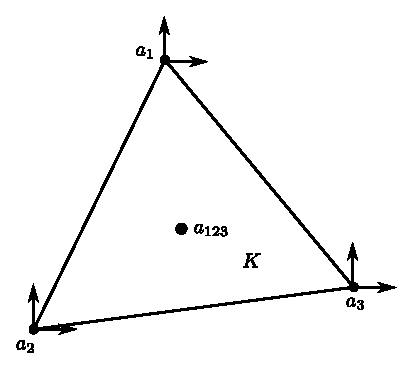
\includegraphics{figures/fig3.8.eps}
\centerline{\bf Fig. 3.8.}
\end{figure}\pageoriginale

\begin{remark*}
Even for this boundary value problem, there is still no existence theorem establishing a weak solution.
\end{remark*}

Let $U^j_i$ represent an approximation for $\phi$ at the mesh poit $x = i \Delta x$, $y = j \Delta y$. The form of difference scheme proposed for the elliptic region is:
\begin{equation*}
\frac{1}{2\Delta x} [(\frac{U^j_{i+1} - U^j_i}{\Delta x})^2 - (\frac{U^j_i - U^j_{i-1}}{\Delta x})^2] + \frac{1}{(\Delta y)^2}  [U^{j+1}_i - 2U^j_i + U^{j-1}_i] =0,  
\tag{3.37}\label{eq3.37}
\end{equation*}
a second order accurate scheme. Note that in this forms the difference analogue of $\oint \phi^2_x dy - \phi_y dx = 0$. This is in so called conservation form. In the hyperbolic region we {\em retard } the $x$-differences and use
\begin{equation*}
\frac{1}{2\Delta x} [(\frac{U^j_i - U^j_{i-1}}{\Delta x})^2 - (\frac{U^j_{i-1} - U^j_{i-2}}{\Delta x})^2] + \frac{1}{(\Delta y)^2 }  [U^{j+1}_{i-1} - 2U^j_{i-1} + U^{j-1}_{i-1}] = 0 \tag{3.38}\label{eq3.38}
\end{equation*}
This is accurate to second order for some equation of the form 
\begin{equation*}
\frac{1}{2} (\phi^2_x)_x + \phi_{yy} = (\epsilon(\phi^2_x)_x)_{x}\tag{3.39}\label{eq3.39}
\end{equation*}\pageoriginale
where $\epsilon =0$ for $\phi_x >0$. The scheme thus introduces {\em articicial dissipation} but only in the supersonic region, cf. Chapter I \S\S\ 5 and 7. 

\begin{exer*}
Investigate the one dimensional form of (\ref{eq3.39}) and see how the solution depends on the parameter. 
\end{exer*}

The object is to prescribe appropriate boundary conditions using (\ref{eq3.36}) and then to solve (\ref{eq3.37}) and (\ref{eq3.38}) for $U^j_i$. For this a particular relaxation method is used which we will interpret as a time dependent problem on the original equation. Consider 
$$
\phi_{xt} = \phi_x \phi_{xx} + \phi_{yy},
$$
with the same boundary conditions. Then solve numerically by differencing the following:
\begin{align*}
\tilde{\phi}_{xt} & = \tilde{\phi}_x \tilde{\phi}_{xx} \quad \text{in} \quad n \Delta t \leqq t \leqq (n+1) \Delta t\tag{3.40}\label{eq3.40}\\
\tilde{\tilde{\phi}}_{xt} & = \tilde{\tilde{\phi}}_{yy} \quad \text{in} \quad (n+1) \Delta t \leqq t \leqq (n+2) \Delta t \tag{3.41}\label{eq3.41}
\end{align*}
Here $\Delta t$ is small. Define
\begin{equation*}
\phi^* = 
\begin{cases}
& \tilde{\phi} \quad \text{in} \quad n \Delta t \leqq t \leqq (n+1) \Delta t\\
& \tilde{\tilde{\phi}} \quad\text{in}\quad (n+1) \Delta t < t \leqq (n+2) \Delta t
\end{cases}\tag{3.42}\label{eq3.42}
\end{equation*}
This is an alternating direction scheme and it turns out that {\em if the quantities are smooth}, this alternate direction scheme implies
$$
\phi^* \to \phi \quad \text{as} \quad \Delta t \to 0.
$$
However,\pageoriginale we do not expect a smooth solution; a shock occurs and across this shock $\phi_x$ increases in accordance with the entropy condition if the difference have been retarded in the $x$ - direction and if the shock can be described by $x = X(y)$. Furthermore one belives that $\phi$ approaches a steady state as $t \to \infty$ and this steady state is the desired solution.

If we now difference the alternating direction time dependent\break scheme
in time and space we get a particular relaxation scheme for finding
$U^j_i$. 

Alternative schemes have been suggested by Engquist, Osher \cite{key9}, who show in fact that there exists a solution for their difference scheme. The main ideas of this method have been used by Jameson \cite{key18} and others to solve the full equations and in recent work the method has been applied to three dimensional flows where the computing difficulties are very great.

\section{Nozzle flow}\label{chap3:sec3.13}
Another transition flow from subsonic to supersonic occurs in a nozzle but with much more stable behaviour.

The simplest example is a Meyer flow (see Bers \cite{key2}) where there is an elegant exact solution. From (\ref{eq3.8}) one finds the equations for $q,\theta$ as functions of $\phi,\psi$ and one finds near $q=c$ that
$$
S_\psi = \theta_\phi, \quad SS_\phi = \theta_\psi,
$$
where $S$ is related to $\sigma$. For every $A$,
\begin{align*}
S & = A \phi + \frac{A^2}{2}  \psi^2\\
\theta & = A^2 \phi \psi + \frac{A^3}{6} \psi^3
\end{align*}\pageoriginale
is a solution. The flow in the $\phi, \psi$ plane has, of course, as streamlines the horizontals $\psi = $ constant. Thus the wall of the corresponding flow in $\phi, \psi$ plane consists of two straight lines.

The sonic line is a parabola and the characteristics are $(\theta - \theta_o)^2 = \dfrac{4}{9} \sigma^3$ and there are four of them passing through $\phi =0$, $\psi =0$ given by $\phi = \pm \dfrac{A}{4} \psi^2$. Hence the mapping into the hodograph plane is not one-to-one but there is a fold and the region $\theta^2 < \dfrac{4}{9} \sigma^3$ is covered {\em three} times.

To design a general nozzle with prescribed speed at infinity, we therefore solve
$$
K\psi_{\theta \theta} + \psi_{\sigma\sigma} =0
$$
in the hodograph plane $\sigma, \theta$. Specify the singularity at $\sigma_\infty$ by analogue with incompressible flow (see the Figure 3.9). Leave out the gap made by the characteristics through the origin.
\begin{figure}[H]
\centering
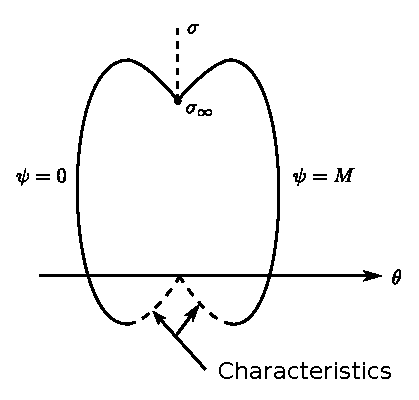
\includegraphics{figures/fig3.9.eps}
\centerline{\bf Fig. 3.9.}
\end{figure}


Next\pageoriginale continue the flow across the characteristics to get two layers ending on the characteristics. Continue the flow on the third sheet into the whole quadrant bounded by four characteristics.

To continue the flow, one uses hyperbolic methods. The flow can be terminated by a shock and the outgoing flow from the nozzle will be subsonic.


\begin{thebibliography}{99}
\bibitem{key1} BAUER, F., GARABEDIAN, P. and KORN, D.,\pageoriginale A Theory of Supercritical Wing Sections with Computer Programs and Examples, Springer--Verlag, (1972) Lecture Notes in Economical and Mathematical Sciences, Vol.66. See also Vol. 108 and 150 in same series. 

\addcontentsline{toc}{chapter}{Bibliography}

\bibitem{key2} BERS, L., Mathematical Aspects of Subsonic and Transonic Gas Dynamics, John Wiley, New York (1958).

\bibitem{key3} BREZIS, H. and STAMPACCHIA, G., The Hodograph Method in Fluid Dynamics in the Light of Variational Inequalities, Arch. Rat. Mech. Ana., 61, 1-18 (1976). 

\bibitem{key4} BRISTEAU, M., GLOWINSKI, R., PERIAUX, J., PERRIER, P., PIRONNEAU, O. and POIRIER, G., Application of Optimal  Control and Finite Element Methods to the Calculation of Transonic Flows and Incompressible Viscous Flows, France, I.R.A. Rep. \# 294 (1978).

\bibitem{key5} COOK, L.P., A Uniqueness Proof for Transonic Flow Problem, Ind. Univ. Math. J., 27, 51-71 (1978).

\bibitem{key6} COURANT, R. and FRIEDRICHS, K.O., Supersonic Flow and Shock Waves, Interscience Publ., New York (1948), reprinted by Springer--Verlag.

\bibitem{key7} CRANDALL, M.G. and TARTAR, L., Some relations between nonexpansive and order preserving mappings, MRC Tech. Rep. \# 1943, Wisconsin (1979).

\bibitem{key8} DIPERNA, R.J., Uniqueness of solutions to Hyperbolic Conservation Laws, Ind. Univ. Math. J., 28, 137-188 (1979).
 
\bibitem{key9} ENGQUIST, B. and OSHER, S.,\pageoriginale Stable and entropy satisfying  approximations for transonic flow calculations, Math. Comp., 34, 45-75 (1980).

\bibitem{key10} FRANKL, F.L., On the formation of shock waves in subsonic flows with local supersonic velocities, Akad. Nauk. SSSR, Prikl. Math. Mech., 11, 199-202 (1947).

\bibitem{key11} FRIEDRICHS, K.O., On the mathematical theory of deflagrations and detonations, United States, Navel Rep. 79-46, Bureau of Ordnance, 1946.

\bibitem{key12} FUNG, K.Y., SOBIECZKY, H. and SEEBASS, R., Shock--Free Wing Design, AIAA Jour. 18, 1153--1158 (1980).

\bibitem{key13} GARABEDIAN, P.R., Partial Differential Equations, John Wiley, New York (1964).

\bibitem{key14} GILBARG, D., Uniqueness of Axially Symmetric Flows with free boundaries, J. Rat. Mech. Ana., 1, 309-320 (1952). 

\bibitem{key15} GLIMM, J., Solutions in the Large for Nonlinear Hyperbolic Systems of Equations, Comm. PUre Appl. Math., 18, 697-715 (1965).

\bibitem{key16} GUDERLEY, G., On the presence of shocks in mixed subsonic supersonic flow patterns, Adv. Appl. Mech. 3, Academic, New York.

\bibitem{key17} HARTEN, A., The Artificial Compression method for computing shocks and contact discontinuities, Comm. Pure. Math., 30, 611-630 (1977).

\bibitem{key18} JAMESON, A., Iterative solution of transonic flows over airfoils and wings, including flows at Mach 1, Ibid, 27, 283-309 (1974).

\bibitem{key19} JOHN, F., Blow-up\pageoriginale or solutions of nonlinear wave equations in threee space dimensions, Manuscript a Mathematica, 28, 235--268 (1979).

\bibitem{key20} KEYFITZ, B., Solutions with shocks; an example of an $L^1$ - contractive semigroup, Comm. Pure. Appl. Math., 24, 125-132 (1971).

\bibitem{key21} KLAINERMAN, S., Global Existence for Nonlinear Wave equations, Ibid., 33, 43-101 (1980).

\bibitem{key22} LAVRENT'EV, M.A. and BITZADZE, A.V., On the problem of equations of the mixed type, Dokl. Akad. SSSR, 70, 373-376 (1954). 

\bibitem{key23} LAX, P.D., Hyperbolic Systems of Conservation Laws and the Mathematical Theory of Shock Waves, SIAM (1973). 

\bibitem{key24} LAX, P.D. and WENDROFF, C., Difference Schemes for Hyperbolic Equations with high order of accuracy, Comm. Pure. Appl. Math., 17, 381-394 (1964).

\bibitem{key25} LIGHTHILL, M.J., The Hodograph Transformation in Transonic Flow, II and III, Proc. Roy. Soc. London, A191, 341-369 (1947).

\bibitem{key26} LIGHTHILL, M.J., and WHITHAM, G.B., On Kinematic waves: I. Flood movement in long rivers; II. Theory of traffic flow on long crowded roads, Proc. Roy. Soc. London, A229, 281-345 (1955).

\bibitem{key27} MORAWETZ, C.S., Mixed Equations and Transonic Flows, Rendiconti di Mat., 25, 1-25 (1966).

\bibitem{key28} MORAWETZ, C.S., Non--Existence of Transonic Flow past a profile, Comm. Pure. Appl. Math., 17, 357-367 (1964).

\bibitem{key29} MORAWETZ, C.S.,\pageoriginale On the Non-Existence of continuous transonic flow past profiles, I, II and III, Comm. Pure. Appl. Math., 9, 45-68 (1956), 10, 107-131 (1957), and 11, 129-144 (1958).

\bibitem{key30}  MORAWETZ, C.S., A weak solution for a system of Equations of Elliptic-Hyperbolic type, Ibid., 11, 315--331 (1958).

\bibitem{key31} MORAWETZ, C.S., The Dirichlet Problem for the Tricomi. Equation, Ibid., 23, 587-601 (1970).

\bibitem{key32} MURMAN, E.M. and COLE, J.D., Calculation of plane steady transonic flows, AIAA Jour., 9, 114-121 (1971).

\bibitem{key33} NIEUWLAND, G.Y., Transonic potential flow around a family of quasi elliptical aerofoil sections, Netherlands, NLR Rep. TR T172 (1967).

\bibitem{key34} OLIENIK, O.A., Uniqueness and stability of the generalised solution of the Cauchy problem for a quasilinear equation, Am. Math. Soc. Transl., 33(2), 285-290 (1965).

\bibitem{key35} OSHER, S., Boundary value problems for equations of mixed type I. The Lavrent'ev-Bitzadze  model, Comm. Partial Diff. Eqns., 2, 499-547 (1977).

\bibitem{key36} TRICOMI, F., Sulle equazioni lineari alle derivate parziali di $2^\circ$ ordine di tipo misto, Atti Accad. Naz. Lincei, Rend., 14, 133-247 (1923). 
\end{thebibliography}
